\documentclass[twoside]{book}

% Packages required by doxygen
\usepackage{calc}
\usepackage{doxygen}
\usepackage{graphicx}
\usepackage[utf8]{inputenc}
\usepackage{makeidx}
\usepackage{multicol}
\usepackage{multirow}
\usepackage{fixltx2e}
\PassOptionsToPackage{warn}{textcomp}
\usepackage{textcomp}
\usepackage[nointegrals]{wasysym}
\usepackage[table]{xcolor}

% Font selection
\usepackage[T1]{fontenc}
\usepackage{mathptmx}
\usepackage[scaled=.90]{helvet}
\usepackage{courier}
\usepackage{amssymb}
\usepackage{sectsty}
\renewcommand{\familydefault}{\sfdefault}
\allsectionsfont{%
  \fontseries{bc}\selectfont%
  \color{darkgray}%
}
\renewcommand{\DoxyLabelFont}{%
  \fontseries{bc}\selectfont%
  \color{darkgray}%
}
\newcommand{\+}{\discretionary{\mbox{\scriptsize$\hookleftarrow$}}{}{}}

% Page & text layout
\usepackage{geometry}
\geometry{%
  a4paper,%
  top=2.5cm,%
  bottom=2.5cm,%
  left=2.5cm,%
  right=2.5cm%
}
\tolerance=750
\hfuzz=15pt
\hbadness=750
\setlength{\emergencystretch}{15pt}
\setlength{\parindent}{0cm}
\setlength{\parskip}{0.2cm}
\makeatletter
\renewcommand{\paragraph}{%
  \@startsection{paragraph}{4}{0ex}{-1.0ex}{1.0ex}{%
    \normalfont\normalsize\bfseries\SS@parafont%
  }%
}
\renewcommand{\subparagraph}{%
  \@startsection{subparagraph}{5}{0ex}{-1.0ex}{1.0ex}{%
    \normalfont\normalsize\bfseries\SS@subparafont%
  }%
}
\makeatother

% Headers & footers
\usepackage{fancyhdr}
\pagestyle{fancyplain}
\fancyhead[LE]{\fancyplain{}{\bfseries\thepage}}
\fancyhead[CE]{\fancyplain{}{}}
\fancyhead[RE]{\fancyplain{}{\bfseries\leftmark}}
\fancyhead[LO]{\fancyplain{}{\bfseries\rightmark}}
\fancyhead[CO]{\fancyplain{}{}}
\fancyhead[RO]{\fancyplain{}{\bfseries\thepage}}
\fancyfoot[LE]{\fancyplain{}{}}
\fancyfoot[CE]{\fancyplain{}{}}
\fancyfoot[RE]{\fancyplain{}{\bfseries\scriptsize Generated on Sun Jun 15 2014 12\+:10\+:29 for My Project by Doxygen }}
\fancyfoot[LO]{\fancyplain{}{\bfseries\scriptsize Generated on Sun Jun 15 2014 12\+:10\+:29 for My Project by Doxygen }}
\fancyfoot[CO]{\fancyplain{}{}}
\fancyfoot[RO]{\fancyplain{}{}}
\renewcommand{\footrulewidth}{0.4pt}
\renewcommand{\chaptermark}[1]{%
  \markboth{#1}{}%
}
\renewcommand{\sectionmark}[1]{%
  \markright{\thesection\ #1}%
}

% Indices & bibliography
\usepackage{natbib}
\usepackage[titles]{tocloft}
\setcounter{tocdepth}{3}
\setcounter{secnumdepth}{5}
\makeindex

% Hyperlinks (required, but should be loaded last)
\usepackage{ifpdf}
\ifpdf
  \usepackage[pdftex,pagebackref=true]{hyperref}
\else
  \usepackage[ps2pdf,pagebackref=true]{hyperref}
\fi
\hypersetup{%
  colorlinks=true,%
  linkcolor=blue,%
  citecolor=blue,%
  unicode%
}

% Custom commands
\newcommand{\clearemptydoublepage}{%
  \newpage{\pagestyle{empty}\cleardoublepage}%
}


%===== C O N T E N T S =====

\begin{document}

% Titlepage & ToC
\hypersetup{pageanchor=false,
             bookmarks=true,
             bookmarksnumbered=true,
             pdfencoding=unicode
            }
\pagenumbering{roman}
\begin{titlepage}
\vspace*{7cm}
\begin{center}%
{\Large My Project }\\
\vspace*{1cm}
{\large Generated by Doxygen 1.8.7}\\
\vspace*{0.5cm}
{\small Sun Jun 15 2014 12:10:29}\\
\end{center}
\end{titlepage}
\clearemptydoublepage
\tableofcontents
\clearemptydoublepage
\pagenumbering{arabic}
\hypersetup{pageanchor=true}

%--- Begin generated contents ---
\chapter{Hierarchical Index}
\section{Class Hierarchy}
This inheritance list is sorted roughly, but not completely, alphabetically\+:\begin{DoxyCompactList}
\item \contentsline{section}{Categorie\+Manager}{\pageref{class_categorie_manager}}{}
\item \contentsline{section}{Dossier}{\pageref{class_dossier}}{}
\item \contentsline{section}{formation}{\pageref{classformation}}{}
\item \contentsline{section}{Note\+Manager}{\pageref{class_note_manager}}{}
\item Q\+Dialog\begin{DoxyCompactList}
\item \contentsline{section}{ajouter\+U\+V\+Window}{\pageref{classajouter_u_v_window}}{}
\item \contentsline{section}{Opening\+Window}{\pageref{class_opening_window}}{}
\end{DoxyCompactList}
\item Q\+Main\+Window\begin{DoxyCompactList}
\item \contentsline{section}{Main\+Window}{\pageref{class_main_window}}{}
\end{DoxyCompactList}
\item \contentsline{section}{Semestre}{\pageref{class_semestre}}{}
\item \contentsline{section}{U\+T\+Profiler\+Exception}{\pageref{class_u_t_profiler_exception}}{}
\item \contentsline{section}{U\+V}{\pageref{class_u_v}}{}
\item \contentsline{section}{U\+V\+Manager}{\pageref{class_u_v_manager}}{}
\end{DoxyCompactList}

\chapter{Class Index}
\section{Class List}
Here are the classes, structs, unions and interfaces with brief descriptions\+:\begin{DoxyCompactList}
\item\contentsline{section}{\hyperlink{classajouter_u_v_window}{ajouter\+U\+V\+Window} }{\pageref{classajouter_u_v_window}}{}
\item\contentsline{section}{\hyperlink{class_categorie_manager}{Categorie\+Manager} \\*The \hyperlink{class_categorie_manager}{Categorie\+Manager} class \hyperlink{class_categorie_manager}{Categorie\+Manager} contient une Q\+Map de 2 Q\+String \+: La première indique le nom abrégé de la catégorie, la 2e son nom complet }{\pageref{class_categorie_manager}}{}
\item\contentsline{section}{\hyperlink{class_dossier}{Dossier} }{\pageref{class_dossier}}{}
\item\contentsline{section}{\hyperlink{classformation}{formation} }{\pageref{classformation}}{}
\item\contentsline{section}{\hyperlink{class_main_window}{Main\+Window} }{\pageref{class_main_window}}{}
\item\contentsline{section}{\hyperlink{class_note_manager}{Note\+Manager} }{\pageref{class_note_manager}}{}
\item\contentsline{section}{\hyperlink{class_opening_window}{Opening\+Window} }{\pageref{class_opening_window}}{}
\item\contentsline{section}{\hyperlink{class_semestre}{Semestre} \\*La classe \hyperlink{class_semestre}{Semestre} construit un \hyperlink{class_semestre}{Semestre} à partir d'une saison et d'une année }{\pageref{class_semestre}}{}
\item\contentsline{section}{\hyperlink{class_u_t_profiler_exception}{U\+T\+Profiler\+Exception} }{\pageref{class_u_t_profiler_exception}}{}
\item\contentsline{section}{\hyperlink{class_u_v}{U\+V} \\*La classe \hyperlink{class_u_v}{U\+V} permet d'enregistrer les différentes informations sur une \hyperlink{class_u_v}{U\+V} }{\pageref{class_u_v}}{}
\item\contentsline{section}{\hyperlink{class_u_v_manager}{U\+V\+Manager} \\*La classe \hyperlink{class_u_v_manager}{U\+V\+Manager} permet de gérer l'ensemble des U\+Vs }{\pageref{class_u_v_manager}}{}
\end{DoxyCompactList}

\chapter{File Index}
\section{File List}
Here is a list of all documented files with brief descriptions\+:\begin{DoxyCompactList}
\item\contentsline{section}{{\bfseries ajouteruvwindow.\+h} }{\pageref{ajouteruvwindow_8h}}{}
\item\contentsline{section}{{\bfseries formationmanager.\+h} }{\pageref{formationmanager_8h}}{}
\item\contentsline{section}{{\bfseries mainwindow.\+h} }{\pageref{mainwindow_8h}}{}
\item\contentsline{section}{{\bfseries openingwindow.\+h} }{\pageref{openingwindow_8h}}{}
\item\contentsline{section}{{\bfseries utprofilerexception.\+h} }{\pageref{utprofilerexception_8h}}{}
\item\contentsline{section}{\hyperlink{uvmanager_8h}{uvmanager.\+h} \\*Header des classes Categories\+Manager et \hyperlink{class_u_v_manager}{U\+V\+Manager} }{\pageref{uvmanager_8h}}{}
\end{DoxyCompactList}

\chapter{Class Documentation}
\hypertarget{classajouter_u_v_window}{\section{ajouter\+U\+V\+Window Class Reference}
\label{classajouter_u_v_window}\index{ajouter\+U\+V\+Window@{ajouter\+U\+V\+Window}}
}
Inheritance diagram for ajouter\+U\+V\+Window\+:\begin{figure}[H]
\begin{center}
\leavevmode
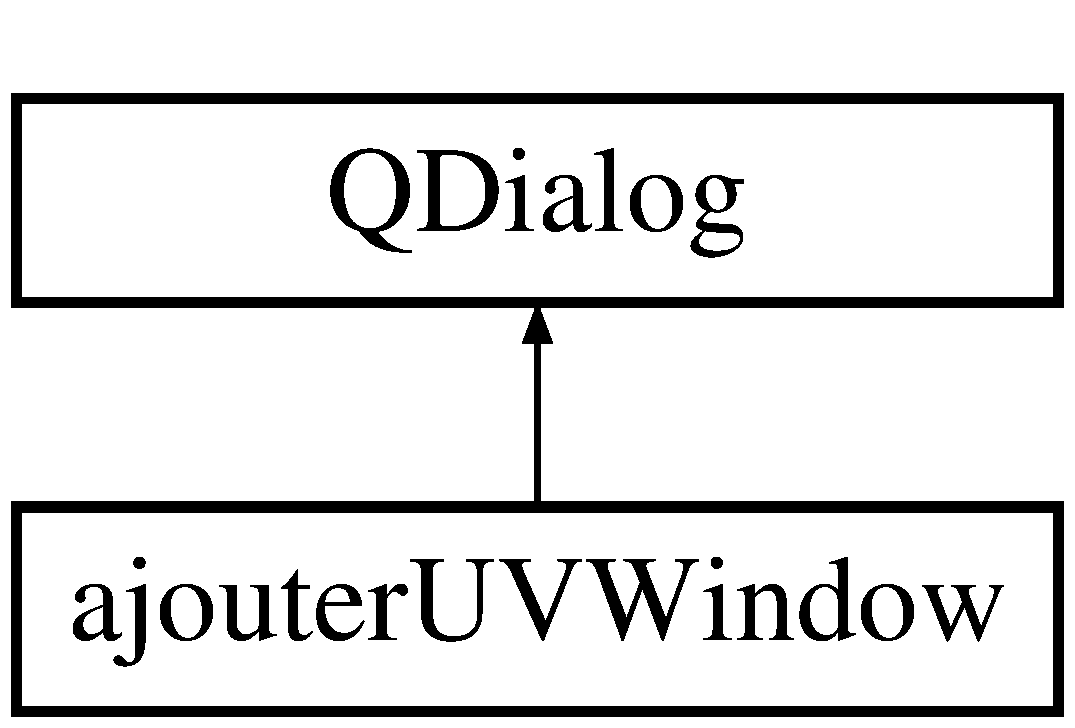
\includegraphics[height=2.000000cm]{classajouter_u_v_window}
\end{center}
\end{figure}
\subsection*{Public Slots}
\begin{DoxyCompactItemize}
\item 
\hypertarget{classajouter_u_v_window_ae420a5021cc1c808cc1829272a3632de}{void {\bfseries on\+\_\+txt\+Code\+New\+U\+V\+\_\+text\+Changed} ()}\label{classajouter_u_v_window_ae420a5021cc1c808cc1829272a3632de}

\item 
\hypertarget{classajouter_u_v_window_a924f5c0bd03bd28d7837fe3db9349a21}{void {\bfseries on\+\_\+txt\+Desc\+New\+U\+V\+\_\+text\+Changed} ()}\label{classajouter_u_v_window_a924f5c0bd03bd28d7837fe3db9349a21}

\item 
\hypertarget{classajouter_u_v_window_ad670ccb53cdaeb7c07672eec2b3750f6}{void {\bfseries U\+V\+Editee} ()}\label{classajouter_u_v_window_ad670ccb53cdaeb7c07672eec2b3750f6}

\item 
\hypertarget{classajouter_u_v_window_ab91685c4fa6df3f269e00ba5ebf11466}{void {\bfseries on\+\_\+btn\+Annuler\+\_\+clicked} ()}\label{classajouter_u_v_window_ab91685c4fa6df3f269e00ba5ebf11466}

\item 
\hypertarget{classajouter_u_v_window_ab427343ed27b3c809c771c35f6c049b7}{void {\bfseries on\+\_\+btn\+Accepter\+\_\+clicked} ()}\label{classajouter_u_v_window_ab427343ed27b3c809c771c35f6c049b7}

\end{DoxyCompactItemize}
\subsection*{Signals}
\begin{DoxyCompactItemize}
\item 
\hypertarget{classajouter_u_v_window_a90c73636da04e8b86282720edba7be74}{void {\bfseries U\+V\+Added} ()}\label{classajouter_u_v_window_a90c73636da04e8b86282720edba7be74}

\end{DoxyCompactItemize}
\subsection*{Public Member Functions}
\begin{DoxyCompactItemize}
\item 
\hypertarget{classajouter_u_v_window_adb410d8cb02f2759f64aeebe8eae337e}{{\bfseries ajouter\+U\+V\+Window} (Q\+Widget $\ast$parent=0)}\label{classajouter_u_v_window_adb410d8cb02f2759f64aeebe8eae337e}

\end{DoxyCompactItemize}


The documentation for this class was generated from the following files\+:\begin{DoxyCompactItemize}
\item 
ajouteruvwindow.\+h\item 
ajouteruvwindow.\+cpp\end{DoxyCompactItemize}

\hypertarget{class_categorie_manager}{\section{Categorie\+Manager Class Reference}
\label{class_categorie_manager}\index{Categorie\+Manager@{Categorie\+Manager}}
}


The \hyperlink{class_categorie_manager}{Categorie\+Manager} class \hyperlink{class_categorie_manager}{Categorie\+Manager} contient une Q\+Map de 2 Q\+String \+: La première indique le nom abrégé de la catégorie, la 2e son nom complet.  




{\ttfamily \#include $<$uvmanager.\+h$>$}

\subsection*{Public Member Functions}
\begin{DoxyCompactItemize}
\item 
void \hyperlink{class_categorie_manager_a0888fdaa33d645eaf2c4e5977f6bf2fc}{add\+Item} (const Q\+String \&code, const Q\+String \&desc)
\begin{DoxyCompactList}\small\item\em add\+Item ajoute une catégorie à la map des catégories /$\ast$$\ast$ $\ast$ \end{DoxyCompactList}\item 
int \hyperlink{class_categorie_manager_a4f3453ebb942d8992570d9ee450d49d7}{remove\+Item} (const Q\+String \&code)
\begin{DoxyCompactList}\small\item\em remove\+Item supprime de la map des catégories la catégorie au nom abrégé passé en paramètre. \end{DoxyCompactList}\item 
Q\+String \& \hyperlink{class_categorie_manager_a97d678b0d5af868af4474d4fc05c9d46}{get\+Desc} (const Q\+String \&code) const 
\begin{DoxyCompactList}\small\item\em get\+Desc retourne le nom complet d'une catégorie au nom abrégé passé en paramètre. \end{DoxyCompactList}\item 
bool \hyperlink{class_categorie_manager_ab8dcf01ac835ddef441b08b44ca10e7d}{is\+Cat} (const Q\+String \&code)
\begin{DoxyCompactList}\small\item\em is\+Cat indique si la catégorie passée en paramètre existe. \end{DoxyCompactList}\item 
const Q\+Map$<$ Q\+String, Q\+String $>$ \& \hyperlink{class_categorie_manager_a96b90ece8d298ec50f3191f97ff2b1f6}{get\+All\+Categories} () const 
\begin{DoxyCompactList}\small\item\em get\+All\+Categories \+: accesseur pour la Q\+Map categories /$\ast$$\ast$ $\ast$ \end{DoxyCompactList}\end{DoxyCompactItemize}
\subsection*{Static Public Member Functions}
\begin{DoxyCompactItemize}
\item 
static \hyperlink{class_categorie_manager}{Categorie\+Manager} \& \hyperlink{class_categorie_manager_ac27223b725ffade86c87d84a4ffddba9}{get\+Instance} ()
\begin{DoxyCompactList}\small\item\em get\+Instance permet de récupérer l'unique instance de \hyperlink{class_categorie_manager}{Categorie\+Manager} \end{DoxyCompactList}\item 
\hypertarget{class_categorie_manager_a90c87f91898c7459a544cda26daad266}{static void \hyperlink{class_categorie_manager_a90c87f91898c7459a544cda26daad266}{liberer\+Instance} ()}\label{class_categorie_manager_a90c87f91898c7459a544cda26daad266}

\begin{DoxyCompactList}\small\item\em liberer\+Instance supprimer l'unique instance de \hyperlink{class_categorie_manager}{Categorie\+Manager} \end{DoxyCompactList}\end{DoxyCompactItemize}
\subsection*{Friends}
\begin{DoxyCompactItemize}
\item 
\hypertarget{class_categorie_manager_a7ab9a1e3d1a8ab9a8badf544bf7e0197}{struct {\bfseries Handler}}\label{class_categorie_manager_a7ab9a1e3d1a8ab9a8badf544bf7e0197}

\end{DoxyCompactItemize}


\subsection{Detailed Description}
The \hyperlink{class_categorie_manager}{Categorie\+Manager} class \hyperlink{class_categorie_manager}{Categorie\+Manager} contient une Q\+Map de 2 Q\+String \+: La première indique le nom abrégé de la catégorie, la 2e son nom complet. 

\subsection{Member Function Documentation}
\hypertarget{class_categorie_manager_a0888fdaa33d645eaf2c4e5977f6bf2fc}{\index{Categorie\+Manager@{Categorie\+Manager}!add\+Item@{add\+Item}}
\index{add\+Item@{add\+Item}!Categorie\+Manager@{Categorie\+Manager}}
\subsubsection[{add\+Item}]{\setlength{\rightskip}{0pt plus 5cm}void Categorie\+Manager\+::add\+Item (
\begin{DoxyParamCaption}
\item[{const Q\+String \&}]{code, }
\item[{const Q\+String \&}]{desc}
\end{DoxyParamCaption}
)}}\label{class_categorie_manager_a0888fdaa33d645eaf2c4e5977f6bf2fc}


add\+Item ajoute une catégorie à la map des catégories /$\ast$$\ast$ $\ast$ 

/$\ast$$\ast$ $\ast$ 
\begin{DoxyParams}{Parameters}
{\em code} & \+: nom abrégé de la catégorie /$\ast$$\ast$ $\ast$ \\
\hline
{\em desc} & \+: nom complet de la catégorie \\
\hline
\end{DoxyParams}
\hypertarget{class_categorie_manager_a96b90ece8d298ec50f3191f97ff2b1f6}{\index{Categorie\+Manager@{Categorie\+Manager}!get\+All\+Categories@{get\+All\+Categories}}
\index{get\+All\+Categories@{get\+All\+Categories}!Categorie\+Manager@{Categorie\+Manager}}
\subsubsection[{get\+All\+Categories}]{\setlength{\rightskip}{0pt plus 5cm}const Q\+Map$<$Q\+String, Q\+String$>$\& Categorie\+Manager\+::get\+All\+Categories (
\begin{DoxyParamCaption}
{}
\end{DoxyParamCaption}
) const\hspace{0.3cm}{\ttfamily [inline]}}}\label{class_categorie_manager_a96b90ece8d298ec50f3191f97ff2b1f6}


get\+All\+Categories \+: accesseur pour la Q\+Map categories /$\ast$$\ast$ $\ast$ 

/$\ast$$\ast$ $\ast$ \begin{DoxyReturn}{Returns}
Q\+Map$<$\+Q\+String, Q\+String$>$ categories 
\end{DoxyReturn}
\hypertarget{class_categorie_manager_a97d678b0d5af868af4474d4fc05c9d46}{\index{Categorie\+Manager@{Categorie\+Manager}!get\+Desc@{get\+Desc}}
\index{get\+Desc@{get\+Desc}!Categorie\+Manager@{Categorie\+Manager}}
\subsubsection[{get\+Desc}]{\setlength{\rightskip}{0pt plus 5cm}Q\+String \& Categorie\+Manager\+::get\+Desc (
\begin{DoxyParamCaption}
\item[{const Q\+String \&}]{code}
\end{DoxyParamCaption}
) const}}\label{class_categorie_manager_a97d678b0d5af868af4474d4fc05c9d46}


get\+Desc retourne le nom complet d'une catégorie au nom abrégé passé en paramètre. 


\begin{DoxyParams}{Parameters}
{\em code} & \+: Nom abrégé de la catégorie \\
\hline
\end{DoxyParams}
\begin{DoxyReturn}{Returns}
Nom complet de la catégorie. 
\end{DoxyReturn}
\hypertarget{class_categorie_manager_ac27223b725ffade86c87d84a4ffddba9}{\index{Categorie\+Manager@{Categorie\+Manager}!get\+Instance@{get\+Instance}}
\index{get\+Instance@{get\+Instance}!Categorie\+Manager@{Categorie\+Manager}}
\subsubsection[{get\+Instance}]{\setlength{\rightskip}{0pt plus 5cm}{\bf Categorie\+Manager} \& Categorie\+Manager\+::get\+Instance (
\begin{DoxyParamCaption}
{}
\end{DoxyParamCaption}
)\hspace{0.3cm}{\ttfamily [static]}}}\label{class_categorie_manager_ac27223b725ffade86c87d84a4ffddba9}


get\+Instance permet de récupérer l'unique instance de \hyperlink{class_categorie_manager}{Categorie\+Manager} 

\begin{DoxyReturn}{Returns}
Instance unique de \hyperlink{class_categorie_manager}{Categorie\+Manager} 
\end{DoxyReturn}
\hypertarget{class_categorie_manager_ab8dcf01ac835ddef441b08b44ca10e7d}{\index{Categorie\+Manager@{Categorie\+Manager}!is\+Cat@{is\+Cat}}
\index{is\+Cat@{is\+Cat}!Categorie\+Manager@{Categorie\+Manager}}
\subsubsection[{is\+Cat}]{\setlength{\rightskip}{0pt plus 5cm}bool Categorie\+Manager\+::is\+Cat (
\begin{DoxyParamCaption}
\item[{const Q\+String \&}]{code}
\end{DoxyParamCaption}
)}}\label{class_categorie_manager_ab8dcf01ac835ddef441b08b44ca10e7d}


is\+Cat indique si la catégorie passée en paramètre existe. 


\begin{DoxyParams}{Parameters}
{\em code} & \+: nom abrégé de la catégorie recherchée. \\
\hline
\end{DoxyParams}
\begin{DoxyReturn}{Returns}
Vrai si la catégorie existe dans la map, faux sinon. 
\end{DoxyReturn}
\hypertarget{class_categorie_manager_a4f3453ebb942d8992570d9ee450d49d7}{\index{Categorie\+Manager@{Categorie\+Manager}!remove\+Item@{remove\+Item}}
\index{remove\+Item@{remove\+Item}!Categorie\+Manager@{Categorie\+Manager}}
\subsubsection[{remove\+Item}]{\setlength{\rightskip}{0pt plus 5cm}int Categorie\+Manager\+::remove\+Item (
\begin{DoxyParamCaption}
\item[{const Q\+String \&}]{code}
\end{DoxyParamCaption}
)}}\label{class_categorie_manager_a4f3453ebb942d8992570d9ee450d49d7}


remove\+Item supprime de la map des catégories la catégorie au nom abrégé passé en paramètre. 


\begin{DoxyParams}{Parameters}
{\em code} & \+: nom abrégé de la catégorie à supprimer. \\
\hline
\end{DoxyParams}
\begin{DoxyReturn}{Returns}
Nombre de catégories supprimées (normalement 1). 
\end{DoxyReturn}


The documentation for this class was generated from the following files\+:\begin{DoxyCompactItemize}
\item 
\hyperlink{uvmanager_8h}{uvmanager.\+h}\item 
uvmanager.\+cpp\end{DoxyCompactItemize}

\hypertarget{class_dossier}{\section{Dossier Class Reference}
\label{class_dossier}\index{Dossier@{Dossier}}
}


The documentation for this class was generated from the following file\+:\begin{DoxyCompactItemize}
\item 
\hyperlink{uvmanager_8h}{uvmanager.\+h}\end{DoxyCompactItemize}

\hypertarget{classformation}{\section{formation Class Reference}
\label{classformation}\index{formation@{formation}}
}
\subsection*{Public Member Functions}
\begin{DoxyCompactItemize}
\item 
\hypertarget{classformation_a49f0c32e0bc38601c725bcdd0a7252e1}{Q\+String {\bfseries get\+Code} () const }\label{classformation_a49f0c32e0bc38601c725bcdd0a7252e1}

\item 
\hypertarget{classformation_aa151fd31c40af7b9d97d4d49f631a127}{Q\+String {\bfseries get\+Titre} () const }\label{classformation_aa151fd31c40af7b9d97d4d49f631a127}

\item 
\hypertarget{classformation_a3b11f669e83ad0d5b72838645b1608aa}{Q\+Map$<$ Q\+String, int $>$ {\bfseries get\+Credits} () const }\label{classformation_a3b11f669e83ad0d5b72838645b1608aa}

\item 
\hypertarget{classformation_a0a803b64845bc0b1a2858e794ce53d6d}{Q\+Set$<$ Q\+String $>$ {\bfseries get\+Formations} () const }\label{classformation_a0a803b64845bc0b1a2858e794ce53d6d}

\item 
\hypertarget{classformation_ae1ebb6483415cbdd45d0b08b64fbc965}{void {\bfseries set\+Code} (const Q\+String \&c)}\label{classformation_ae1ebb6483415cbdd45d0b08b64fbc965}

\item 
\hypertarget{classformation_afe8a4194dcf2fb84034103a352261b88}{void {\bfseries set\+Titre} (const Q\+String \&t)}\label{classformation_afe8a4194dcf2fb84034103a352261b88}

\item 
\hypertarget{classformation_ae602dff10220ef6dc3a8ccb000d40b07}{void {\bfseries set\+Credit} (Q\+String cat, int nb\+C)}\label{classformation_ae602dff10220ef6dc3a8ccb000d40b07}

\item 
\hypertarget{classformation_ac080e767e63497ba274149876e34af57}{void {\bfseries set\+Formation} (Q\+String \hyperlink{classformation}{formation})}\label{classformation_ac080e767e63497ba274149876e34af57}

\end{DoxyCompactItemize}
\subsection*{Friends}
\begin{DoxyCompactItemize}
\item 
\hypertarget{classformation_a2c2226dacc6a09e4f390cda4bdc76eba}{class {\bfseries formation\+Manager}}\label{classformation_a2c2226dacc6a09e4f390cda4bdc76eba}

\end{DoxyCompactItemize}


The documentation for this class was generated from the following file\+:\begin{DoxyCompactItemize}
\item 
formationmanager.\+h\end{DoxyCompactItemize}

\hypertarget{class_main_window}{\section{Main\+Window Class Reference}
\label{class_main_window}\index{Main\+Window@{Main\+Window}}
}
Inheritance diagram for Main\+Window\+:\begin{figure}[H]
\begin{center}
\leavevmode
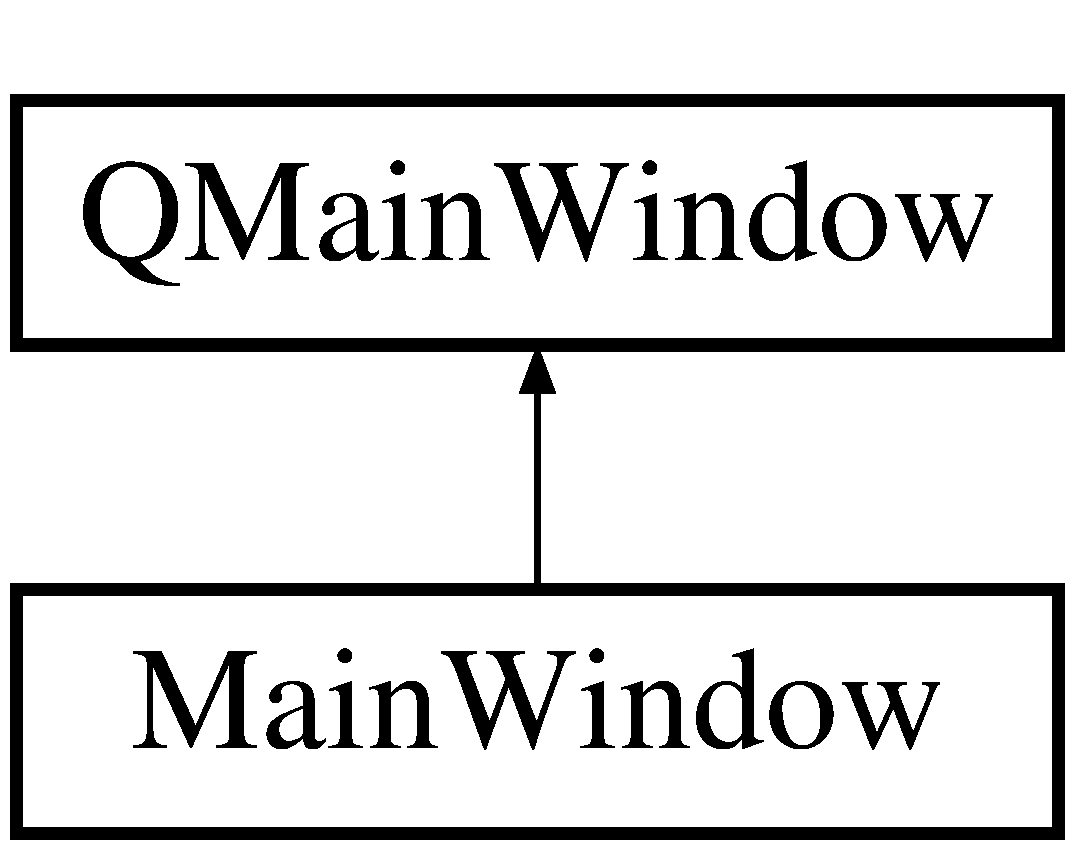
\includegraphics[height=2.000000cm]{class_main_window}
\end{center}
\end{figure}
\subsection*{Public Slots}
\begin{DoxyCompactItemize}
\item 
\hypertarget{class_main_window_aceb6eba1c65888d08f243d2b28807598}{void {\bfseries on\+\_\+action\+Choisir\+\_\+le\+\_\+fichier\+\_\+des\+\_\+\+U\+V\+\_\+triggered} ()}\label{class_main_window_aceb6eba1c65888d08f243d2b28807598}

\item 
\hypertarget{class_main_window_af778a098b79c929ae29486be827192af}{void {\bfseries on\+\_\+action\+Charger\+\_\+un\+\_\+nouveau\+\_\+fichier\+\_\+formations\+\_\+triggered} ()}\label{class_main_window_af778a098b79c929ae29486be827192af}

\item 
\hypertarget{class_main_window_a94b47d9008454ea1c0911d4c74de780a}{void {\bfseries on\+\_\+action\+Dossier\+\_\+\+Etudiant\+\_\+triggered} ()}\label{class_main_window_a94b47d9008454ea1c0911d4c74de780a}

\item 
\hypertarget{class_main_window_afe9d9d46e61e2460e636619577a9e8fd}{void {\bfseries on\+\_\+action\+Quitter\+\_\+triggered} ()}\label{class_main_window_afe9d9d46e61e2460e636619577a9e8fd}

\item 
\hypertarget{class_main_window_adffb9d15a6eefe9d5c6296fc57e6aeab}{void {\bfseries on\+\_\+list\+U\+V\+\_\+current\+Index\+Changed} ()}\label{class_main_window_adffb9d15a6eefe9d5c6296fc57e6aeab}

\item 
\hypertarget{class_main_window_a858a38f003089560d1c8c2506a7cc8c7}{void {\bfseries on\+\_\+txt\+Code\+U\+V\+\_\+text\+Changed} ()}\label{class_main_window_a858a38f003089560d1c8c2506a7cc8c7}

\item 
\hypertarget{class_main_window_ae48298b981c4dcbd136c228a2b0343af}{void {\bfseries on\+\_\+txt\+Description\+\_\+text\+Changed} ()}\label{class_main_window_ae48298b981c4dcbd136c228a2b0343af}

\item 
\hypertarget{class_main_window_af96bb132d657e4795f0d9e9ea31af6ad}{void {\bfseries on\+\_\+chk\+Automne\+\_\+state\+Changed} ()}\label{class_main_window_af96bb132d657e4795f0d9e9ea31af6ad}

\item 
\hypertarget{class_main_window_a0033bd1e6cdcd07e7e395a12665735c6}{void {\bfseries on\+\_\+chk\+Printemps\+\_\+state\+Changed} ()}\label{class_main_window_a0033bd1e6cdcd07e7e395a12665735c6}

\item 
\hypertarget{class_main_window_a6b9781cf986867f8937450a59c3be108}{void {\bfseries on\+\_\+table\+Credits\+\_\+clicked} ()}\label{class_main_window_a6b9781cf986867f8937450a59c3be108}

\item 
\hypertarget{class_main_window_a584c187beaa5a10db5a0a0dcf23bb94a}{void {\bfseries U\+V\+Editee} ()}\label{class_main_window_a584c187beaa5a10db5a0a0dcf23bb94a}

\item 
\hypertarget{class_main_window_a19a34bba77b784a84a5e1ddc02b070c5}{void {\bfseries refresh\+U\+V\+List} ()}\label{class_main_window_a19a34bba77b784a84a5e1ddc02b070c5}

\item 
\hypertarget{class_main_window_a99ae5b77512a4af864c7a3978a2e9c68}{void {\bfseries on\+\_\+btn\+Sauver\+U\+V\+\_\+clicked} ()}\label{class_main_window_a99ae5b77512a4af864c7a3978a2e9c68}

\item 
\hypertarget{class_main_window_a08296ae696d74f8608b443e7f518bc2b}{void {\bfseries on\+\_\+btn\+Ajouter\+U\+V\+\_\+clicked} ()}\label{class_main_window_a08296ae696d74f8608b443e7f518bc2b}

\item 
\hypertarget{class_main_window_ad62fa3cd85fdb2b06723f609809df5a1}{void {\bfseries on\+\_\+btn\+Delete\+U\+V\+\_\+clicked} ()}\label{class_main_window_ad62fa3cd85fdb2b06723f609809df5a1}

\item 
\hypertarget{class_main_window_af90c95ef7c164471f5901371da6e5dda}{void {\bfseries on\+\_\+action\+Save\+U\+V\+\_\+triggered} ()}\label{class_main_window_af90c95ef7c164471f5901371da6e5dda}

\item 
\hypertarget{class_main_window_a42052ea3e95394a8de3b2763047aefaa}{void {\bfseries on\+\_\+action\+Save\+Tous\+\_\+les\+\_\+fichiers\+\_\+triggered} ()}\label{class_main_window_a42052ea3e95394a8de3b2763047aefaa}

\end{DoxyCompactItemize}
\subsection*{Public Member Functions}
\begin{DoxyCompactItemize}
\item 
\hypertarget{class_main_window_a8b244be8b7b7db1b08de2a2acb9409db}{{\bfseries Main\+Window} (Q\+Widget $\ast$parent=0)}\label{class_main_window_a8b244be8b7b7db1b08de2a2acb9409db}

\end{DoxyCompactItemize}
\subsection*{Protected Member Functions}
\begin{DoxyCompactItemize}
\item 
\hypertarget{class_main_window_a4e20a4a065fbb0e4d3532a45a0a91425}{void {\bfseries close\+Event} (Q\+Close\+Event $\ast$event)}\label{class_main_window_a4e20a4a065fbb0e4d3532a45a0a91425}

\end{DoxyCompactItemize}


The documentation for this class was generated from the following files\+:\begin{DoxyCompactItemize}
\item 
mainwindow.\+h\item 
mainwindow.\+cpp\end{DoxyCompactItemize}

\hypertarget{class_note_manager}{\section{Note\+Manager Class Reference}
\label{class_note_manager}\index{Note\+Manager@{Note\+Manager}}
}
\subsection*{Public Member Functions}
\begin{DoxyCompactItemize}
\item 
\hypertarget{class_note_manager_a43de96f6bc9295fd889f90e37aff4381}{void {\bfseries add\+Item} (const Q\+String \&code)}\label{class_note_manager_a43de96f6bc9295fd889f90e37aff4381}

\item 
\hypertarget{class_note_manager_a16d9795a6d44f980e918fecc76d686db}{int {\bfseries remove\+Item} (const Q\+String \&code)}\label{class_note_manager_a16d9795a6d44f980e918fecc76d686db}

\item 
\hypertarget{class_note_manager_aada7f7636665af83c08c5d6bb7a04888}{bool {\bfseries is\+Note} (const Q\+String \&code)}\label{class_note_manager_aada7f7636665af83c08c5d6bb7a04888}

\end{DoxyCompactItemize}
\subsection*{Static Public Member Functions}
\begin{DoxyCompactItemize}
\item 
\hypertarget{class_note_manager_a66d09f446993085eee7b322ec8b289f1}{static \hyperlink{class_note_manager}{Note\+Manager} \& {\bfseries get\+Instance} ()}\label{class_note_manager_a66d09f446993085eee7b322ec8b289f1}

\item 
\hypertarget{class_note_manager_a0ea94a35039be554d8398e01ff5476d6}{static void {\bfseries liberer\+Instance} ()}\label{class_note_manager_a0ea94a35039be554d8398e01ff5476d6}

\end{DoxyCompactItemize}
\subsection*{Friends}
\begin{DoxyCompactItemize}
\item 
\hypertarget{class_note_manager_a7ab9a1e3d1a8ab9a8badf544bf7e0197}{struct {\bfseries Handler}}\label{class_note_manager_a7ab9a1e3d1a8ab9a8badf544bf7e0197}

\end{DoxyCompactItemize}


The documentation for this class was generated from the following files\+:\begin{DoxyCompactItemize}
\item 
\hyperlink{uvmanager_8h}{uvmanager.\+h}\item 
uvmanager.\+cpp\end{DoxyCompactItemize}

\hypertarget{class_opening_window}{\section{Opening\+Window Class Reference}
\label{class_opening_window}\index{Opening\+Window@{Opening\+Window}}
}
Inheritance diagram for Opening\+Window\+:\begin{figure}[H]
\begin{center}
\leavevmode
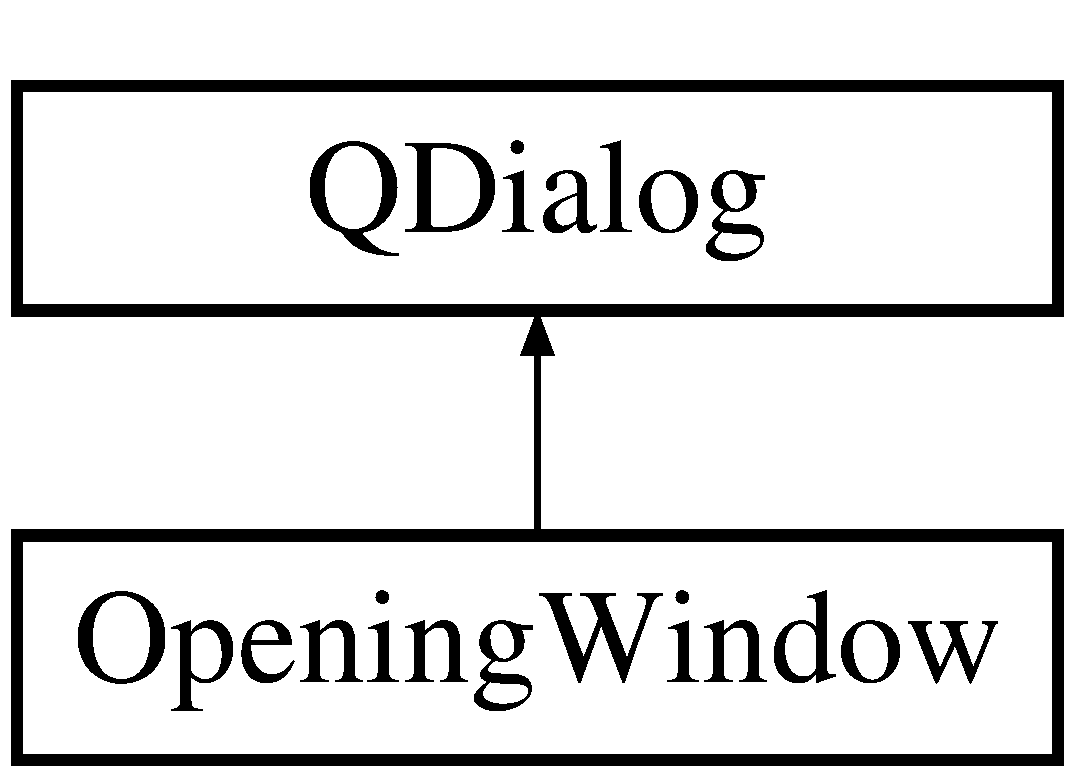
\includegraphics[height=2.000000cm]{class_opening_window}
\end{center}
\end{figure}
\subsection*{Public Slots}
\begin{DoxyCompactItemize}
\item 
\hypertarget{class_opening_window_ad907bae806ede3093d7728ae241d339b}{void {\bfseries on\+\_\+btn\+Parcourir\+U\+V\+\_\+clicked} ()}\label{class_opening_window_ad907bae806ede3093d7728ae241d339b}

\item 
\hypertarget{class_opening_window_a9567830af2746733276c62ce6f7b5e8e}{void {\bfseries on\+\_\+btn\+Valider\+\_\+clicked} ()}\label{class_opening_window_a9567830af2746733276c62ce6f7b5e8e}

\end{DoxyCompactItemize}
\subsection*{Public Member Functions}
\begin{DoxyCompactItemize}
\item 
\hypertarget{class_opening_window_a0ddf01651a723d237c90a541d7b0c79b}{{\bfseries Opening\+Window} (Q\+Widget $\ast$parent=0)}\label{class_opening_window_a0ddf01651a723d237c90a541d7b0c79b}

\end{DoxyCompactItemize}


The documentation for this class was generated from the following files\+:\begin{DoxyCompactItemize}
\item 
openingwindow.\+h\item 
openingwindow.\+cpp\end{DoxyCompactItemize}

\hypertarget{class_semestre}{\section{Semestre Class Reference}
\label{class_semestre}\index{Semestre@{Semestre}}
}


La classe \hyperlink{class_semestre}{Semestre} construit un \hyperlink{class_semestre}{Semestre} à partir d'une saison et d'une année.  




{\ttfamily \#include $<$uvmanager.\+h$>$}

\subsection*{Public Member Functions}
\begin{DoxyCompactItemize}
\item 
\hyperlink{class_semestre_a4a0f1d3ab2f65755e0e0f610526522c2}{Semestre} (\hyperlink{uvmanager_8h_a72fcaae0ef529616dd62b747e259d545}{Saison} s, unsigned int a)
\begin{DoxyCompactList}\small\item\em Constructeur de la classe \hyperlink{class_semestre}{Semestre}. \end{DoxyCompactList}\item 
\hyperlink{uvmanager_8h_a72fcaae0ef529616dd62b747e259d545}{Saison} \hyperlink{class_semestre_a26e25575e7fb65649c47970a9800c3aa}{get\+Saison} () const 
\begin{DoxyCompactList}\small\item\em get\+Saison \+: accesseur sur Saison \end{DoxyCompactList}\item 
unsigned int \hyperlink{class_semestre_a5aa85395e97f58f491ebf251da8231ef}{get\+Annee} () const 
\begin{DoxyCompactList}\small\item\em get\+Annee \+: accesseur sur Année. \end{DoxyCompactList}\end{DoxyCompactItemize}


\subsection{Detailed Description}
La classe \hyperlink{class_semestre}{Semestre} construit un \hyperlink{class_semestre}{Semestre} à partir d'une saison et d'une année. 

\subsection{Constructor \& Destructor Documentation}
\hypertarget{class_semestre_a4a0f1d3ab2f65755e0e0f610526522c2}{\index{Semestre@{Semestre}!Semestre@{Semestre}}
\index{Semestre@{Semestre}!Semestre@{Semestre}}
\subsubsection[{Semestre}]{\setlength{\rightskip}{0pt plus 5cm}Semestre\+::\+Semestre (
\begin{DoxyParamCaption}
\item[{{\bf Saison}}]{s, }
\item[{unsigned int}]{a}
\end{DoxyParamCaption}
)\hspace{0.3cm}{\ttfamily [inline]}}}\label{class_semestre_a4a0f1d3ab2f65755e0e0f610526522c2}


Constructeur de la classe \hyperlink{class_semestre}{Semestre}. 


\begin{DoxyParams}{Parameters}
{\em s} & \+: Saison (automne ou printemps) \\
\hline
{\em a} & \+: année entre 1972 et 2099. \\
\hline
\end{DoxyParams}


\subsection{Member Function Documentation}
\hypertarget{class_semestre_a5aa85395e97f58f491ebf251da8231ef}{\index{Semestre@{Semestre}!get\+Annee@{get\+Annee}}
\index{get\+Annee@{get\+Annee}!Semestre@{Semestre}}
\subsubsection[{get\+Annee}]{\setlength{\rightskip}{0pt plus 5cm}unsigned int Semestre\+::get\+Annee (
\begin{DoxyParamCaption}
{}
\end{DoxyParamCaption}
) const\hspace{0.3cm}{\ttfamily [inline]}}}\label{class_semestre_a5aa85395e97f58f491ebf251da8231ef}


get\+Annee \+: accesseur sur Année. 

\begin{DoxyReturn}{Returns}
Année du \hyperlink{class_semestre}{Semestre}. 
\end{DoxyReturn}
\hypertarget{class_semestre_a26e25575e7fb65649c47970a9800c3aa}{\index{Semestre@{Semestre}!get\+Saison@{get\+Saison}}
\index{get\+Saison@{get\+Saison}!Semestre@{Semestre}}
\subsubsection[{get\+Saison}]{\setlength{\rightskip}{0pt plus 5cm}{\bf Saison} Semestre\+::get\+Saison (
\begin{DoxyParamCaption}
{}
\end{DoxyParamCaption}
) const\hspace{0.3cm}{\ttfamily [inline]}}}\label{class_semestre_a26e25575e7fb65649c47970a9800c3aa}


get\+Saison \+: accesseur sur Saison 

\begin{DoxyReturn}{Returns}
Saison du \hyperlink{class_semestre}{Semestre}. 
\end{DoxyReturn}


The documentation for this class was generated from the following file\+:\begin{DoxyCompactItemize}
\item 
\hyperlink{uvmanager_8h}{uvmanager.\+h}\end{DoxyCompactItemize}

\hypertarget{class_u_t_profiler_exception}{\section{U\+T\+Profiler\+Exception Class Reference}
\label{class_u_t_profiler_exception}\index{U\+T\+Profiler\+Exception@{U\+T\+Profiler\+Exception}}
}
\subsection*{Public Member Functions}
\begin{DoxyCompactItemize}
\item 
\hypertarget{class_u_t_profiler_exception_afd289268648bada41417156ceb1269fd}{{\bfseries U\+T\+Profiler\+Exception} (const Q\+String \&message, const Q\+String \&f=\char`\"{}na\char`\"{}, unsigned int l=0)}\label{class_u_t_profiler_exception_afd289268648bada41417156ceb1269fd}

\item 
\hypertarget{class_u_t_profiler_exception_a6f4582234c00b4fe67776ef10c5370bf}{Q\+String {\bfseries get\+Info} () const }\label{class_u_t_profiler_exception_a6f4582234c00b4fe67776ef10c5370bf}

\item 
\hypertarget{class_u_t_profiler_exception_ae54e6a5c0836dcc62fee879651ae5679}{Q\+String {\bfseries get\+File} () const }\label{class_u_t_profiler_exception_ae54e6a5c0836dcc62fee879651ae5679}

\item 
\hypertarget{class_u_t_profiler_exception_aa3c2efb28c6b482859b26b8f59b4b32e}{unsigned int {\bfseries get\+Line} () const }\label{class_u_t_profiler_exception_aa3c2efb28c6b482859b26b8f59b4b32e}

\end{DoxyCompactItemize}


The documentation for this class was generated from the following file\+:\begin{DoxyCompactItemize}
\item 
utprofilerexception.\+h\end{DoxyCompactItemize}

\hypertarget{class_u_v}{\section{U\+V Class Reference}
\label{class_u_v}\index{U\+V@{U\+V}}
}


La classe \hyperlink{class_u_v}{U\+V} permet d'enregistrer les différentes informations sur une \hyperlink{class_u_v}{U\+V}.  




{\ttfamily \#include $<$uvmanager.\+h$>$}

\subsection*{Public Member Functions}
\begin{DoxyCompactItemize}
\item 
Q\+String \hyperlink{class_u_v_a4d5fe39505b3e474b41013dda0d2047a}{get\+Code} () const 
\begin{DoxyCompactList}\small\item\em Accesseur sur le code de l'\hyperlink{class_u_v}{U\+V}. \end{DoxyCompactList}\item 
Q\+String \hyperlink{class_u_v_afa7f5a8c7ea21bedcd00af1a1ff48221}{get\+Titre} () const 
\begin{DoxyCompactList}\small\item\em Accesseur sur le titre de l'\hyperlink{class_u_v}{U\+V}. \end{DoxyCompactList}\item 
unsigned int \hyperlink{class_u_v_aca0cf43b1b3b5a7060b21a65fb5701c2}{get\+Nb\+Credits} (Q\+String cat) const 
\begin{DoxyCompactList}\small\item\em get\+Nb\+Credits renvoie le nombre de crédits de l'\hyperlink{class_u_v}{U\+V} pour une catégorie donnée. \end{DoxyCompactList}\item 
unsigned int \hyperlink{class_u_v_a9f95880400dac05e2d18513826062b14}{get\+Nb\+Credits\+Total} () const 
\begin{DoxyCompactList}\small\item\em get\+Nb\+Credits\+Total calcule le nombre total des crédits attribués avec l'obtention de l'\hyperlink{class_u_v}{U\+V}. \end{DoxyCompactList}\item 
Q\+Map$<$ Q\+String, int $>$ \hyperlink{class_u_v_ac9e4b2f7e639ac8d96d01fc8a33a730f}{get\+Categories} () const 
\begin{DoxyCompactList}\small\item\em Accesseur sur les catégories de l'\hyperlink{class_u_v}{U\+V}. \end{DoxyCompactList}\item 
bool \hyperlink{class_u_v_a29423fb485037fc882b8b29cae033c9a}{ouverture\+Automne} () const 
\begin{DoxyCompactList}\small\item\em L'\hyperlink{class_u_v}{U\+V} ouvre-\/t-\/elle à l'automne ? \end{DoxyCompactList}\item 
bool \hyperlink{class_u_v_adca45078b74fdc3c09621a521756e8af}{ouverture\+Printemps} () const 
\begin{DoxyCompactList}\small\item\em L'\hyperlink{class_u_v}{U\+V} ouvre-\/t-\/elle au printemps ? \end{DoxyCompactList}\item 
void \hyperlink{class_u_v_a9c3b73077819774423559abd838e410b}{set\+Code} (const Q\+String \&c)
\begin{DoxyCompactList}\small\item\em Setter sur le code de l'\hyperlink{class_u_v}{U\+V}. \end{DoxyCompactList}\item 
void \hyperlink{class_u_v_a52c66013e137689883802465596bb688}{set\+Titre} (const Q\+String \&t)
\begin{DoxyCompactList}\small\item\em Setter sur le titre de l'\hyperlink{class_u_v}{U\+V}. \end{DoxyCompactList}\item 
void \hyperlink{class_u_v_a6310e1d779721ce541aaea845f205dd1}{set\+Categorie} (Q\+String cat, int nb\+C)
\begin{DoxyCompactList}\small\item\em Setter pour l'insertion de crédits d'une catégorie. \end{DoxyCompactList}\item 
void \hyperlink{class_u_v_a7e670e649febebe0fe70c3ce79f4be63}{set\+Ouverture\+Automne} (bool b)
\begin{DoxyCompactList}\small\item\em set\+Ouverture\+Automne ouvre ou non l'\hyperlink{class_u_v}{U\+V} à l'automne. \end{DoxyCompactList}\item 
void \hyperlink{class_u_v_a0ae246826809cc48a1999ec0671c78b3}{set\+Ouverture\+Printemps} (bool b)
\begin{DoxyCompactList}\small\item\em set\+Ouverture\+Printemps ouvre ou non l'\hyperlink{class_u_v}{U\+V} au printemps. \end{DoxyCompactList}\end{DoxyCompactItemize}
\subsection*{Friends}
\begin{DoxyCompactItemize}
\item 
\hypertarget{class_u_v_a335ec2026467669b89518b0c67372f3b}{class {\bfseries U\+V\+Manager}}\label{class_u_v_a335ec2026467669b89518b0c67372f3b}

\end{DoxyCompactItemize}


\subsection{Detailed Description}
La classe \hyperlink{class_u_v}{U\+V} permet d'enregistrer les différentes informations sur une \hyperlink{class_u_v}{U\+V}. 

\subsection{Member Function Documentation}
\hypertarget{class_u_v_ac9e4b2f7e639ac8d96d01fc8a33a730f}{\index{U\+V@{U\+V}!get\+Categories@{get\+Categories}}
\index{get\+Categories@{get\+Categories}!U\+V@{U\+V}}
\subsubsection[{get\+Categories}]{\setlength{\rightskip}{0pt plus 5cm}Q\+Map$<$Q\+String, int$>$ U\+V\+::get\+Categories (
\begin{DoxyParamCaption}
{}
\end{DoxyParamCaption}
) const\hspace{0.3cm}{\ttfamily [inline]}}}\label{class_u_v_ac9e4b2f7e639ac8d96d01fc8a33a730f}


Accesseur sur les catégories de l'\hyperlink{class_u_v}{U\+V}. 

\begin{DoxyReturn}{Returns}
Q\+Map des catégories de l'\hyperlink{class_u_v}{U\+V}. 
\end{DoxyReturn}
\hypertarget{class_u_v_a4d5fe39505b3e474b41013dda0d2047a}{\index{U\+V@{U\+V}!get\+Code@{get\+Code}}
\index{get\+Code@{get\+Code}!U\+V@{U\+V}}
\subsubsection[{get\+Code}]{\setlength{\rightskip}{0pt plus 5cm}Q\+String U\+V\+::get\+Code (
\begin{DoxyParamCaption}
{}
\end{DoxyParamCaption}
) const\hspace{0.3cm}{\ttfamily [inline]}}}\label{class_u_v_a4d5fe39505b3e474b41013dda0d2047a}


Accesseur sur le code de l'\hyperlink{class_u_v}{U\+V}. 

\begin{DoxyReturn}{Returns}
Code de l'\hyperlink{class_u_v}{U\+V}. 
\end{DoxyReturn}
\hypertarget{class_u_v_aca0cf43b1b3b5a7060b21a65fb5701c2}{\index{U\+V@{U\+V}!get\+Nb\+Credits@{get\+Nb\+Credits}}
\index{get\+Nb\+Credits@{get\+Nb\+Credits}!U\+V@{U\+V}}
\subsubsection[{get\+Nb\+Credits}]{\setlength{\rightskip}{0pt plus 5cm}unsigned int U\+V\+::get\+Nb\+Credits (
\begin{DoxyParamCaption}
\item[{Q\+String}]{cat}
\end{DoxyParamCaption}
) const\hspace{0.3cm}{\ttfamily [inline]}}}\label{class_u_v_aca0cf43b1b3b5a7060b21a65fb5701c2}


get\+Nb\+Credits renvoie le nombre de crédits de l'\hyperlink{class_u_v}{U\+V} pour une catégorie donnée. 


\begin{DoxyParams}{Parameters}
{\em cat} & \+: code de la catégorie. \\
\hline
\end{DoxyParams}
\begin{DoxyReturn}{Returns}
Nombre de crédits attribués dans la catégorie. 
\end{DoxyReturn}
\hypertarget{class_u_v_a9f95880400dac05e2d18513826062b14}{\index{U\+V@{U\+V}!get\+Nb\+Credits\+Total@{get\+Nb\+Credits\+Total}}
\index{get\+Nb\+Credits\+Total@{get\+Nb\+Credits\+Total}!U\+V@{U\+V}}
\subsubsection[{get\+Nb\+Credits\+Total}]{\setlength{\rightskip}{0pt plus 5cm}unsigned int U\+V\+::get\+Nb\+Credits\+Total (
\begin{DoxyParamCaption}
{}
\end{DoxyParamCaption}
) const}}\label{class_u_v_a9f95880400dac05e2d18513826062b14}


get\+Nb\+Credits\+Total calcule le nombre total des crédits attribués avec l'obtention de l'\hyperlink{class_u_v}{U\+V}. 

\begin{DoxyReturn}{Returns}
Somme des crédits des catégories concernées par l'\hyperlink{class_u_v}{U\+V}. 
\end{DoxyReturn}
\hypertarget{class_u_v_afa7f5a8c7ea21bedcd00af1a1ff48221}{\index{U\+V@{U\+V}!get\+Titre@{get\+Titre}}
\index{get\+Titre@{get\+Titre}!U\+V@{U\+V}}
\subsubsection[{get\+Titre}]{\setlength{\rightskip}{0pt plus 5cm}Q\+String U\+V\+::get\+Titre (
\begin{DoxyParamCaption}
{}
\end{DoxyParamCaption}
) const\hspace{0.3cm}{\ttfamily [inline]}}}\label{class_u_v_afa7f5a8c7ea21bedcd00af1a1ff48221}


Accesseur sur le titre de l'\hyperlink{class_u_v}{U\+V}. 

\begin{DoxyReturn}{Returns}
Titre de l'\hyperlink{class_u_v}{U\+V}. 
\end{DoxyReturn}
\hypertarget{class_u_v_a29423fb485037fc882b8b29cae033c9a}{\index{U\+V@{U\+V}!ouverture\+Automne@{ouverture\+Automne}}
\index{ouverture\+Automne@{ouverture\+Automne}!U\+V@{U\+V}}
\subsubsection[{ouverture\+Automne}]{\setlength{\rightskip}{0pt plus 5cm}bool U\+V\+::ouverture\+Automne (
\begin{DoxyParamCaption}
{}
\end{DoxyParamCaption}
) const\hspace{0.3cm}{\ttfamily [inline]}}}\label{class_u_v_a29423fb485037fc882b8b29cae033c9a}


L'\hyperlink{class_u_v}{U\+V} ouvre-\/t-\/elle à l'automne ? 

\begin{DoxyReturn}{Returns}
Vrai si c'est le cas, faux sinon. 
\end{DoxyReturn}
\hypertarget{class_u_v_adca45078b74fdc3c09621a521756e8af}{\index{U\+V@{U\+V}!ouverture\+Printemps@{ouverture\+Printemps}}
\index{ouverture\+Printemps@{ouverture\+Printemps}!U\+V@{U\+V}}
\subsubsection[{ouverture\+Printemps}]{\setlength{\rightskip}{0pt plus 5cm}bool U\+V\+::ouverture\+Printemps (
\begin{DoxyParamCaption}
{}
\end{DoxyParamCaption}
) const\hspace{0.3cm}{\ttfamily [inline]}}}\label{class_u_v_adca45078b74fdc3c09621a521756e8af}


L'\hyperlink{class_u_v}{U\+V} ouvre-\/t-\/elle au printemps ? 

\begin{DoxyReturn}{Returns}
Vrai si c'est le cas, faux sinon. 
\end{DoxyReturn}
\hypertarget{class_u_v_a6310e1d779721ce541aaea845f205dd1}{\index{U\+V@{U\+V}!set\+Categorie@{set\+Categorie}}
\index{set\+Categorie@{set\+Categorie}!U\+V@{U\+V}}
\subsubsection[{set\+Categorie}]{\setlength{\rightskip}{0pt plus 5cm}void U\+V\+::set\+Categorie (
\begin{DoxyParamCaption}
\item[{Q\+String}]{cat, }
\item[{int}]{nb\+C}
\end{DoxyParamCaption}
)\hspace{0.3cm}{\ttfamily [inline]}}}\label{class_u_v_a6310e1d779721ce541aaea845f205dd1}


Setter pour l'insertion de crédits d'une catégorie. 


\begin{DoxyParams}{Parameters}
{\em cat} & \+: Catégorie concernée. \\
\hline
{\em nb\+C} & \+: Nombre de crédits alloués par l'\hyperlink{class_u_v}{U\+V} dans la catégorie. \\
\hline
\end{DoxyParams}
\hypertarget{class_u_v_a9c3b73077819774423559abd838e410b}{\index{U\+V@{U\+V}!set\+Code@{set\+Code}}
\index{set\+Code@{set\+Code}!U\+V@{U\+V}}
\subsubsection[{set\+Code}]{\setlength{\rightskip}{0pt plus 5cm}void U\+V\+::set\+Code (
\begin{DoxyParamCaption}
\item[{const Q\+String \&}]{c}
\end{DoxyParamCaption}
)\hspace{0.3cm}{\ttfamily [inline]}}}\label{class_u_v_a9c3b73077819774423559abd838e410b}


Setter sur le code de l'\hyperlink{class_u_v}{U\+V}. 


\begin{DoxyParams}{Parameters}
{\em c} & \+: nouveau code de l'\hyperlink{class_u_v}{U\+V} \\
\hline
\end{DoxyParams}
\hypertarget{class_u_v_a7e670e649febebe0fe70c3ce79f4be63}{\index{U\+V@{U\+V}!set\+Ouverture\+Automne@{set\+Ouverture\+Automne}}
\index{set\+Ouverture\+Automne@{set\+Ouverture\+Automne}!U\+V@{U\+V}}
\subsubsection[{set\+Ouverture\+Automne}]{\setlength{\rightskip}{0pt plus 5cm}void U\+V\+::set\+Ouverture\+Automne (
\begin{DoxyParamCaption}
\item[{bool}]{b}
\end{DoxyParamCaption}
)\hspace{0.3cm}{\ttfamily [inline]}}}\label{class_u_v_a7e670e649febebe0fe70c3ce79f4be63}


set\+Ouverture\+Automne ouvre ou non l'\hyperlink{class_u_v}{U\+V} à l'automne. 


\begin{DoxyParams}{Parameters}
{\em b} & \+: vrai pour l'ouverture, faux sinon. \\
\hline
\end{DoxyParams}
\hypertarget{class_u_v_a0ae246826809cc48a1999ec0671c78b3}{\index{U\+V@{U\+V}!set\+Ouverture\+Printemps@{set\+Ouverture\+Printemps}}
\index{set\+Ouverture\+Printemps@{set\+Ouverture\+Printemps}!U\+V@{U\+V}}
\subsubsection[{set\+Ouverture\+Printemps}]{\setlength{\rightskip}{0pt plus 5cm}void U\+V\+::set\+Ouverture\+Printemps (
\begin{DoxyParamCaption}
\item[{bool}]{b}
\end{DoxyParamCaption}
)\hspace{0.3cm}{\ttfamily [inline]}}}\label{class_u_v_a0ae246826809cc48a1999ec0671c78b3}


set\+Ouverture\+Printemps ouvre ou non l'\hyperlink{class_u_v}{U\+V} au printemps. 


\begin{DoxyParams}{Parameters}
{\em b} & \+: vrai pour l'ouverture, faux sinon. \\
\hline
\end{DoxyParams}
\hypertarget{class_u_v_a52c66013e137689883802465596bb688}{\index{U\+V@{U\+V}!set\+Titre@{set\+Titre}}
\index{set\+Titre@{set\+Titre}!U\+V@{U\+V}}
\subsubsection[{set\+Titre}]{\setlength{\rightskip}{0pt plus 5cm}void U\+V\+::set\+Titre (
\begin{DoxyParamCaption}
\item[{const Q\+String \&}]{t}
\end{DoxyParamCaption}
)\hspace{0.3cm}{\ttfamily [inline]}}}\label{class_u_v_a52c66013e137689883802465596bb688}


Setter sur le titre de l'\hyperlink{class_u_v}{U\+V}. 


\begin{DoxyParams}{Parameters}
{\em t} & \+: nouveau titre de l'\hyperlink{class_u_v}{U\+V}. \\
\hline
\end{DoxyParams}


The documentation for this class was generated from the following files\+:\begin{DoxyCompactItemize}
\item 
\hyperlink{uvmanager_8h}{uvmanager.\+h}\item 
uvmanager.\+cpp\end{DoxyCompactItemize}

\hypertarget{class_u_v_manager}{\section{U\+V\+Manager Class Reference}
\label{class_u_v_manager}\index{U\+V\+Manager@{U\+V\+Manager}}
}


La classe \hyperlink{class_u_v_manager}{U\+V\+Manager} permet de gérer l'ensemble des U\+Vs.  




{\ttfamily \#include $<$uvmanager.\+h$>$}

\subsection*{Public Member Functions}
\begin{DoxyCompactItemize}
\item 
\hypertarget{class_u_v_manager_a60556f66f72f41786ffb70f066f1a846}{void {\bfseries load} (const Q\+String \&f)}\label{class_u_v_manager_a60556f66f72f41786ffb70f066f1a846}

\item 
\hypertarget{class_u_v_manager_a1e52ce1b69c6239d19016ec3cb74bd1c}{void {\bfseries save} (const Q\+String \&f)}\label{class_u_v_manager_a1e52ce1b69c6239d19016ec3cb74bd1c}

\item 
\hypertarget{class_u_v_manager_a40043a0cc0ae5153600c76220ce76f52}{void {\bfseries add\+U\+V} (const Q\+String \&c, const Q\+String \&t, Q\+Map$<$ Q\+String, int $>$ cat, bool a, bool p)}\label{class_u_v_manager_a40043a0cc0ae5153600c76220ce76f52}

\item 
\hypertarget{class_u_v_manager_ab1f7e555b456dd2d34907061f65b1405}{void {\bfseries delete\+U\+V} (const Q\+String \&c)}\label{class_u_v_manager_ab1f7e555b456dd2d34907061f65b1405}

\item 
\hypertarget{class_u_v_manager_ac1a6b93630bb709b33aff7cba798044d}{const \hyperlink{class_u_v}{U\+V} \& {\bfseries get\+U\+V} (const Q\+String \&code) const }\label{class_u_v_manager_ac1a6b93630bb709b33aff7cba798044d}

\item 
\hypertarget{class_u_v_manager_a00f95b40d834d93f0fe326e1a00649a4}{\hyperlink{class_u_v}{U\+V} \& {\bfseries get\+U\+V} (const Q\+String \&code)}\label{class_u_v_manager_a00f95b40d834d93f0fe326e1a00649a4}

\item 
\hypertarget{class_u_v_manager_a0d65e0ea79cf14c5d92b1013805be42a}{const Q\+Map$<$ Q\+String, \hyperlink{class_u_v}{U\+V} $\ast$ $>$ \& {\bfseries get\+All\+U\+V} () const }\label{class_u_v_manager_a0d65e0ea79cf14c5d92b1013805be42a}

\item 
\hypertarget{class_u_v_manager_a95333fbf72dee3874c2e6492969dbfac}{void {\bfseries delete\+All\+U\+V} ()}\label{class_u_v_manager_a95333fbf72dee3874c2e6492969dbfac}

\item 
\hypertarget{class_u_v_manager_a17d95c67bc2d1f4c9d850fb0b9c42262}{\hyperlink{class_categorie_manager}{Categorie\+Manager} \& {\bfseries get\+Categorie\+Manager} () const }\label{class_u_v_manager_a17d95c67bc2d1f4c9d850fb0b9c42262}

\item 
\hypertarget{class_u_v_manager_af1118627f6a08c3ae828f7d46e683e06}{const \hyperlink{class_note_manager}{Note\+Manager} \& {\bfseries get\+Note\+Manager} () const }\label{class_u_v_manager_af1118627f6a08c3ae828f7d46e683e06}

\end{DoxyCompactItemize}
\subsection*{Static Public Member Functions}
\begin{DoxyCompactItemize}
\item 
\hypertarget{class_u_v_manager_a68d219c83584116722ceb5fea3813e12}{static \hyperlink{class_u_v_manager}{U\+V\+Manager} \& {\bfseries get\+Instance} ()}\label{class_u_v_manager_a68d219c83584116722ceb5fea3813e12}

\item 
\hypertarget{class_u_v_manager_abc80aed5b064c9ba0894f41305490052}{static void {\bfseries liberer\+Instance} ()}\label{class_u_v_manager_abc80aed5b064c9ba0894f41305490052}

\end{DoxyCompactItemize}
\subsection*{Public Attributes}
\begin{DoxyCompactItemize}
\item 
\hypertarget{class_u_v_manager_ace844550b9018b15815e04d3b5c115c4}{Q\+String {\bfseries file}}\label{class_u_v_manager_ace844550b9018b15815e04d3b5c115c4}

\end{DoxyCompactItemize}
\subsection*{Friends}
\begin{DoxyCompactItemize}
\item 
\hypertarget{class_u_v_manager_a7ab9a1e3d1a8ab9a8badf544bf7e0197}{struct {\bfseries Handler}}\label{class_u_v_manager_a7ab9a1e3d1a8ab9a8badf544bf7e0197}

\end{DoxyCompactItemize}


\subsection{Detailed Description}
La classe \hyperlink{class_u_v_manager}{U\+V\+Manager} permet de gérer l'ensemble des U\+Vs. 

The documentation for this class was generated from the following files\+:\begin{DoxyCompactItemize}
\item 
\hyperlink{uvmanager_8h}{uvmanager.\+h}\item 
uvmanager.\+cpp\end{DoxyCompactItemize}

\chapter{File Documentation}
\hypertarget{uvmanager_8h}{\section{uvmanager.\+h File Reference}
\label{uvmanager_8h}\index{uvmanager.\+h@{uvmanager.\+h}}
}


Header des classes Categories\+Manager et \hyperlink{class_u_v_manager}{U\+V\+Manager}.  


{\ttfamily \#include \char`\"{}utprofilerexception.\+h\char`\"{}}\\*
{\ttfamily \#include $<$Q\+String$>$}\\*
{\ttfamily \#include $<$Q\+Text\+Stream$>$}\\*
{\ttfamily \#include $<$Q\+Map$>$}\\*
{\ttfamily \#include $<$Q\+Set$>$}\\*
\subsection*{Classes}
\begin{DoxyCompactItemize}
\item 
class \hyperlink{class_categorie_manager}{Categorie\+Manager}
\begin{DoxyCompactList}\small\item\em The \hyperlink{class_categorie_manager}{Categorie\+Manager} class \hyperlink{class_categorie_manager}{Categorie\+Manager} contient une Q\+Map de 2 Q\+String \+: La première indique le nom abrégé de la catégorie, la 2e son nom complet. \end{DoxyCompactList}\item 
class \hyperlink{class_note_manager}{Note\+Manager}
\item 
class \hyperlink{class_semestre}{Semestre}
\begin{DoxyCompactList}\small\item\em La classe \hyperlink{class_semestre}{Semestre} construit un \hyperlink{class_semestre}{Semestre} à partir d'une saison et d'une année. \end{DoxyCompactList}\item 
class \hyperlink{class_u_v}{U\+V}
\begin{DoxyCompactList}\small\item\em La classe \hyperlink{class_u_v}{U\+V} permet d'enregistrer les différentes informations sur une \hyperlink{class_u_v}{U\+V}. \end{DoxyCompactList}\item 
class \hyperlink{class_u_v_manager}{U\+V\+Manager}
\begin{DoxyCompactList}\small\item\em La classe \hyperlink{class_u_v_manager}{U\+V\+Manager} permet de gérer l'ensemble des U\+Vs. \end{DoxyCompactList}\item 
class \hyperlink{class_dossier}{Dossier}
\end{DoxyCompactItemize}
\subsection*{Enumerations}
\begin{DoxyCompactItemize}
\item 
\hypertarget{uvmanager_8h_a72fcaae0ef529616dd62b747e259d545}{enum \hyperlink{uvmanager_8h_a72fcaae0ef529616dd62b747e259d545}{Saison} \{ {\bfseries Automne}, 
{\bfseries Printemps}
 \}}\label{uvmanager_8h_a72fcaae0ef529616dd62b747e259d545}

\begin{DoxyCompactList}\small\item\em Saison est une énumération des 2 saisons possible pour nommer un semestre \+: Automne et Printemps. \end{DoxyCompactList}\end{DoxyCompactItemize}


\subsection{Detailed Description}
Header des classes Categories\+Manager et \hyperlink{class_u_v_manager}{U\+V\+Manager}. 

\begin{DoxyAuthor}{Author}
Clément F\+I\+C\+H\+M\+A\+N\+N et Alexandre K\+E\+I\+L 
\end{DoxyAuthor}
\begin{DoxyDate}{Date}
Juin 2014 
\end{DoxyDate}

%--- End generated contents ---

% Index
\newpage
\phantomsection
\addcontentsline{toc}{chapter}{Index}
\printindex

\end{document}
